\documentclass[1p]{elsarticle_modified}
%\bibliographystyle{elsarticle-num}

%\usepackage[colorlinks]{hyperref}
%\usepackage{abbrmath_seonhwa} %\Abb, \Ascr, \Acal ,\Abf, \Afrak
\usepackage{amsfonts}
\usepackage{amssymb}
\usepackage{amsmath}
\usepackage{amsthm}
\usepackage{scalefnt}
\usepackage{amsbsy}
\usepackage{kotex}
\usepackage{caption}
\usepackage{subfig}
\usepackage{color}
\usepackage{graphicx}
\usepackage{xcolor} %% white, black, red, green, blue, cyan, magenta, yellow
\usepackage{float}
\usepackage{setspace}
\usepackage{hyperref}

\usepackage{tikz}
\usetikzlibrary{arrows}

\usepackage{multirow}
\usepackage{array} % fixed length table
\usepackage{hhline}

%%%%%%%%%%%%%%%%%%%%%
\makeatletter
\renewcommand*\env@matrix[1][\arraystretch]{%
	\edef\arraystretch{#1}%
	\hskip -\arraycolsep
	\let\@ifnextchar\new@ifnextchar
	\array{*\c@MaxMatrixCols c}}
\makeatother %https://tex.stackexchange.com/questions/14071/how-can-i-increase-the-line-spacing-in-a-matrix
%%%%%%%%%%%%%%%

\usepackage[normalem]{ulem}

\newcommand{\msout}[1]{\ifmmode\text{\sout{\ensuremath{#1}}}\else\sout{#1}\fi}
%SOURCE: \msout is \stkout macro in https://tex.stackexchange.com/questions/20609/strikeout-in-math-mode

\newcommand{\cancel}[1]{
	\ifmmode
	{\color{red}\msout{#1}}
	\else
	{\color{red}\sout{#1}}
	\fi
}

\newcommand{\add}[1]{
	{\color{blue}\uwave{#1}}
}

\newcommand{\replace}[2]{
	\ifmmode
	{\color{red}\msout{#1}}{\color{blue}\uwave{#2}}
	\else
	{\color{red}\sout{#1}}{\color{blue}\uwave{#2}}
	\fi
}

\newcommand{\Sol}{\mathcal{S}} %segment
\newcommand{\D}{D} %diagram
\newcommand{\A}{\mathcal{A}} %arc


%%%%%%%%%%%%%%%%%%%%%%%%%%%%%5 test

\def\sl{\operatorname{\textup{SL}}(2,\Cbb)}
\def\psl{\operatorname{\textup{PSL}}(2,\Cbb)}
\def\quan{\mkern 1mu \triangleright \mkern 1mu}

\theoremstyle{definition}
\newtheorem{thm}{Theorem}[section]
\newtheorem{prop}[thm]{Proposition}
\newtheorem{lem}[thm]{Lemma}
\newtheorem{ques}[thm]{Question}
\newtheorem{cor}[thm]{Corollary}
\newtheorem{defn}[thm]{Definition}
\newtheorem{exam}[thm]{Example}
\newtheorem{rmk}[thm]{Remark}
\newtheorem{alg}[thm]{Algorithm}

\newcommand{\I}{\sqrt{-1}}
\begin{document}

%\begin{frontmatter}
%
%\title{Boundary parabolic representations of knots up to 8 crossings}
%
%%% Group authors per affiliation:
%\author{Yunhi Cho} 
%\address{Department of Mathematics, University of Seoul, Seoul, Korea}
%\ead{yhcho@uos.ac.kr}
%
%
%\author{Seonhwa Kim} %\fnref{s_kim}}
%\address{Center for Geometry and Physics, Institute for Basic Science, Pohang, 37673, Korea}
%\ead{ryeona17@ibs.re.kr}
%
%\author{Hyuk Kim}
%\address{Department of Mathematical Sciences, Seoul National University, Seoul 08826, Korea}
%\ead{hyukkim@snu.ac.kr}
%
%\author{Seokbeom Yoon}
%\address{Department of Mathematical Sciences, Seoul National University, Seoul, 08826,  Korea}
%\ead{sbyoon15@snu.ac.kr}
%
%\begin{abstract}
%We find all boundary parabolic representation of knots up to 8 crossings.
%
%\end{abstract}
%\begin{keyword}
%    \MSC[2010] 57M25 
%\end{keyword}
%
%\end{frontmatter}

%\linenumbers
%\tableofcontents
%
\newcommand\colored[1]{\textcolor{white}{\rule[-0.35ex]{0.8em}{1.4ex}}\kern-0.8em\color{red} #1}%
%\newcommand\colored[1]{\textcolor{white}{ #1}\kern-2.17ex	\textcolor{white}{ #1}\kern-1.81ex	\textcolor{white}{ #1}\kern-2.15ex\color{red}#1	}

{\Large $\underline{12n_{0633}~(K12n_{0633})}$}

\setlength{\tabcolsep}{10pt}
\renewcommand{\arraystretch}{1.6}
\vspace{1cm}\begin{tabular}{m{100pt}>{\centering\arraybackslash}m{274pt}}
\multirow{5}{120pt}{
	\centering
	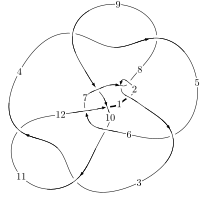
\includegraphics[width=112pt]{../../../GIT/diagram.site/Diagrams/png/2722_12n_0633.png}\\
\ \ \ A knot diagram\footnotemark}&
\allowdisplaybreaks
\textbf{Linearized knot diagam} \\
\cline{2-2}
 &
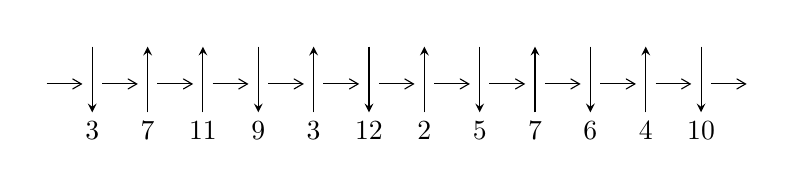
\begin{tikzpicture}[x=20pt, y=17pt]
	% nodes
	\node (C0) at (0, 0) {};
	\node (C1) at (1, 0) {};
	\node (C1U) at (1, +1) {};
	\node (C1D) at (1, -1) {3};

	\node (C2) at (2, 0) {};
	\node (C2U) at (2, +1) {};
	\node (C2D) at (2, -1) {7};

	\node (C3) at (3, 0) {};
	\node (C3U) at (3, +1) {};
	\node (C3D) at (3, -1) {11};

	\node (C4) at (4, 0) {};
	\node (C4U) at (4, +1) {};
	\node (C4D) at (4, -1) {9};

	\node (C5) at (5, 0) {};
	\node (C5U) at (5, +1) {};
	\node (C5D) at (5, -1) {3};

	\node (C6) at (6, 0) {};
	\node (C6U) at (6, +1) {};
	\node (C6D) at (6, -1) {12};

	\node (C7) at (7, 0) {};
	\node (C7U) at (7, +1) {};
	\node (C7D) at (7, -1) {2};

	\node (C8) at (8, 0) {};
	\node (C8U) at (8, +1) {};
	\node (C8D) at (8, -1) {5};

	\node (C9) at (9, 0) {};
	\node (C9U) at (9, +1) {};
	\node (C9D) at (9, -1) {7};

	\node (C10) at (10, 0) {};
	\node (C10U) at (10, +1) {};
	\node (C10D) at (10, -1) {6};

	\node (C11) at (11, 0) {};
	\node (C11U) at (11, +1) {};
	\node (C11D) at (11, -1) {4};

	\node (C12) at (12, 0) {};
	\node (C12U) at (12, +1) {};
	\node (C12D) at (12, -1) {10};
	\node (C13) at (13, 0) {};

	% arrows
	\draw[->,>={angle 60}]
	(C0) edge (C1) (C1) edge (C2) (C2) edge (C3) (C3) edge (C4) (C4) edge (C5) (C5) edge (C6) (C6) edge (C7) (C7) edge (C8) (C8) edge (C9) (C9) edge (C10) (C10) edge (C11) (C11) edge (C12) (C12) edge (C13) ;	\draw[->,>=stealth]
	(C1U) edge (C1D) (C2D) edge (C2U) (C3D) edge (C3U) (C4U) edge (C4D) (C5D) edge (C5U) (C6U) edge (C6D) (C7D) edge (C7U) (C8U) edge (C8D) (C9D) edge (C9U) (C10U) edge (C10D) (C11D) edge (C11U) (C12U) edge (C12D) ;
	\end{tikzpicture} \\
\hhline{~~} \\& 
\textbf{Solving Sequence} \\ \cline{2-2} 
 &
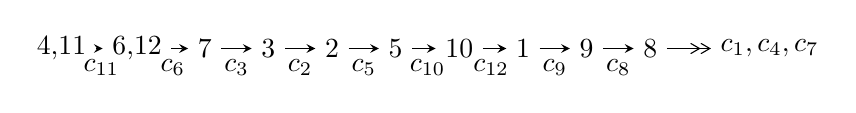
\begin{tikzpicture}[x=23pt, y=7pt]
	% node
	\node (A0) at (-1/8, 0) {4,11};
	\node (A1) at (17/16, 0) {6,12};
	\node (A2) at (17/8, 0) {7};
	\node (A3) at (25/8, 0) {3};
	\node (A4) at (33/8, 0) {2};
	\node (A5) at (41/8, 0) {5};
	\node (A6) at (49/8, 0) {10};
	\node (A7) at (57/8, 0) {1};
	\node (A8) at (65/8, 0) {9};
	\node (A9) at (73/8, 0) {8};
	\node (C1) at (1/2, -1) {$c_{11}$};
	\node (C2) at (13/8, -1) {$c_{6}$};
	\node (C3) at (21/8, -1) {$c_{3}$};
	\node (C4) at (29/8, -1) {$c_{2}$};
	\node (C5) at (37/8, -1) {$c_{5}$};
	\node (C6) at (45/8, -1) {$c_{10}$};
	\node (C7) at (53/8, -1) {$c_{12}$};
	\node (C8) at (61/8, -1) {$c_{9}$};
	\node (C9) at (69/8, -1) {$c_{8}$};
	\node (A10) at (11, 0) {$c_{1},c_{4},c_{7}$};

	% edge
	\draw[->,>=stealth]	
	(A0) edge (A1) (A1) edge (A2) (A2) edge (A3) (A3) edge (A4) (A4) edge (A5) (A5) edge (A6) (A6) edge (A7) (A7) edge (A8) (A8) edge (A9) ;
	\draw[->>,>={angle 60}]	
	(A9) edge (A10);
\end{tikzpicture} \\ 

\end{tabular} \\

\footnotetext{
The image of knot diagram is generated by the software ``\textbf{Draw programme}" developed by Andrew Bartholomew(\url{http://www.layer8.co.uk/maths/draw/index.htm\#Running-draw}), where we modified some parts for our purpose(\url{https://github.com/CATsTAILs/LinksPainter}).
}\phantom \\ \newline 
\centering \textbf{Ideals for irreducible components\footnotemark of $X_{\text{par}}$} 
 
\begin{align*}
I^u_{1}&=\langle 
-6.85653\times10^{96} u^{67}+6.21801\times10^{96} u^{66}+\cdots+1.94852\times10^{96} b-2.56391\times10^{97},\\
\phantom{I^u_{1}}&\phantom{= \langle  }-1.98079\times10^{97} u^{67}+7.40641\times10^{96} u^{66}+\cdots+3.89704\times10^{96} a-1.25871\times10^{98},\\
\phantom{I^u_{1}}&\phantom{= \langle  }u^{68}-21 u^{66}+\cdots-22 u+4\rangle \\
I^u_{2}&=\langle 
34763 u^{19}-7407 u^{18}+\cdots+3686 b-174428,\;-171203 u^{19}+58379 u^{18}+\cdots+7372 a+755094,\\
\phantom{I^u_{2}}&\phantom{= \langle  }u^{20}- u^{19}+\cdots-2 u+4\rangle \\
\\
\end{align*}
\raggedright * 2 irreducible components of $\dim_{\mathbb{C}}=0$, with total 88 representations.\\
\footnotetext{All coefficients of polynomials are rational numbers. But the coefficients are sometimes approximated in decimal forms when there is not enough margin.}
\newpage
\renewcommand{\arraystretch}{1}
\centering \section*{I. $I^u_{1}= \langle -6.86\times10^{96} u^{67}+6.22\times10^{96} u^{66}+\cdots+1.95\times10^{96} b-2.56\times10^{97},\;-1.98\times10^{97} u^{67}+7.41\times10^{96} u^{66}+\cdots+3.90\times10^{96} a-1.26\times10^{98},\;u^{68}-21 u^{66}+\cdots-22 u+4 \rangle$}
\flushleft \textbf{(i) Arc colorings}\\
\begin{tabular}{m{7pt} m{180pt} m{7pt} m{180pt} }
\flushright $a_{4}=$&$\begin{pmatrix}0\\u\end{pmatrix}$ \\
\flushright $a_{11}=$&$\begin{pmatrix}1\\0\end{pmatrix}$ \\
\flushright $a_{6}=$&$\begin{pmatrix}5.08280 u^{67}-1.90052 u^{66}+\cdots-261.858 u+32.2991\\3.51883 u^{67}-3.19114 u^{66}+\cdots-67.4259 u+13.1583\end{pmatrix}$ \\
\flushright $a_{12}=$&$\begin{pmatrix}1\\- u^2\end{pmatrix}$ \\
\flushright $a_{7}=$&$\begin{pmatrix}0.913294 u^{67}+1.61910 u^{66}+\cdots-132.289 u+11.5387\\6.79407 u^{67}-5.84784 u^{66}+\cdots-161.535 u+27.2367\end{pmatrix}$ \\
\flushright $a_{3}=$&$\begin{pmatrix}- u\\u\end{pmatrix}$ \\
\flushright $a_{2}=$&$\begin{pmatrix}16.8822 u^{67}-10.5665 u^{66}+\cdots-538.941 u+75.0706\\-9.25794 u^{67}+6.53626 u^{66}+\cdots+329.727 u-48.4229\end{pmatrix}$ \\
\flushright $a_{5}=$&$\begin{pmatrix}1.71831 u^{67}-0.0689445 u^{66}+\cdots-115.435 u+11.9324\\6.88332 u^{67}-5.02272 u^{66}+\cdots-213.849 u+33.5249\end{pmatrix}$ \\
\flushright $a_{10}=$&$\begin{pmatrix}25.1621 u^{67}-18.4497 u^{66}+\cdots-888.032 u+134.487\\-17.8873 u^{67}+13.8599 u^{66}+\cdots+648.982 u-96.7041\end{pmatrix}$ \\
\flushright $a_{1}=$&$\begin{pmatrix}19.3375 u^{67}-11.7232 u^{66}+\cdots-658.103 u+91.1915\\-11.7133 u^{67}+7.69295 u^{66}+\cdots+448.888 u-64.5438\end{pmatrix}$ \\
\flushright $a_{9}=$&$\begin{pmatrix}-4.85415 u^{67}+4.02937 u^{66}+\cdots+67.1858 u-6.11337\\28.8964 u^{67}-27.6860 u^{66}+\cdots-747.269 u+114.575\end{pmatrix}$ \\
\flushright $a_{8}=$&$\begin{pmatrix}8.95388 u^{67}-5.32862 u^{66}+\cdots-419.793 u+66.1754\\22.8262 u^{67}-22.4977 u^{66}+\cdots-524.537 u+80.1631\end{pmatrix}$\\&\end{tabular}
\flushleft \textbf{(ii) Obstruction class $= -1$}\\~\\
\flushleft \textbf{(iii) Cusp Shapes $= 292.431 u^{67}-245.607 u^{66}+\cdots-9342.95 u+1389.56$}\\~\\
\newpage\renewcommand{\arraystretch}{1}
\flushleft \textbf{(iv) u-Polynomials at the component}\newline \\
\begin{tabular}{m{50pt}|m{274pt}}
Crossings & \hspace{64pt}u-Polynomials at each crossing \\
\hline $$\begin{aligned}c_{1}\end{aligned}$$&$\begin{aligned}
&u^{68}+74 u^{67}+\cdots+5731546 u+418609
\end{aligned}$\\
\hline $$\begin{aligned}c_{2},c_{7}\end{aligned}$$&$\begin{aligned}
&u^{68}+37 u^{66}+\cdots-3274 u+647
\end{aligned}$\\
\hline $$\begin{aligned}c_{3},c_{11}\end{aligned}$$&$\begin{aligned}
&u^{68}-21 u^{66}+\cdots+22 u+4
\end{aligned}$\\
\hline $$\begin{aligned}c_{4},c_{8}\end{aligned}$$&$\begin{aligned}
&u^{68}- u^{67}+\cdots-11 u+1
\end{aligned}$\\
\hline $$\begin{aligned}c_{5}\end{aligned}$$&$\begin{aligned}
&u^{68}+15 u^{66}+\cdots+135093 u+1093
\end{aligned}$\\
\hline $$\begin{aligned}c_{6}\end{aligned}$$&$\begin{aligned}
&u^{68}+u^{67}+\cdots-16 u^2+1
\end{aligned}$\\
\hline $$\begin{aligned}c_{9}\end{aligned}$$&$\begin{aligned}
&u^{68}+5 u^{67}+\cdots+52344 u+5441
\end{aligned}$\\
\hline $$\begin{aligned}c_{10}\end{aligned}$$&$\begin{aligned}
&u^{68}+2 u^{67}+\cdots-82 u+23
\end{aligned}$\\
\hline $$\begin{aligned}c_{12}\end{aligned}$$&$\begin{aligned}
&u^{68}-10 u^{67}+\cdots-74106 u+4643
\end{aligned}$\\
\hline
\end{tabular}\\~\\
\newpage\renewcommand{\arraystretch}{1}
\flushleft \textbf{(v) Riley Polynomials at the component}\newline \\
\begin{tabular}{m{50pt}|m{274pt}}
Crossings & \hspace{64pt}Riley Polynomials at each crossing \\
\hline $$\begin{aligned}c_{1}\end{aligned}$$&$\begin{aligned}
&y^{68}-138 y^{67}+\cdots+15388310151698 y+175233494881
\end{aligned}$\\
\hline $$\begin{aligned}c_{2},c_{7}\end{aligned}$$&$\begin{aligned}
&y^{68}+74 y^{67}+\cdots+5731546 y+418609
\end{aligned}$\\
\hline $$\begin{aligned}c_{3},c_{11}\end{aligned}$$&$\begin{aligned}
&y^{68}-42 y^{67}+\cdots-428 y+16
\end{aligned}$\\
\hline $$\begin{aligned}c_{4},c_{8}\end{aligned}$$&$\begin{aligned}
&y^{68}+9 y^{67}+\cdots-13 y+1
\end{aligned}$\\
\hline $$\begin{aligned}c_{5}\end{aligned}$$&$\begin{aligned}
&y^{68}+30 y^{67}+\cdots-20226072467 y+1194649
\end{aligned}$\\
\hline $$\begin{aligned}c_{6}\end{aligned}$$&$\begin{aligned}
&y^{68}-3 y^{67}+\cdots-32 y+1
\end{aligned}$\\
\hline $$\begin{aligned}c_{9}\end{aligned}$$&$\begin{aligned}
&y^{68}+97 y^{67}+\cdots+2711378272 y+29604481
\end{aligned}$\\
\hline $$\begin{aligned}c_{10}\end{aligned}$$&$\begin{aligned}
&y^{68}+70 y^{66}+\cdots+6570 y+529
\end{aligned}$\\
\hline $$\begin{aligned}c_{12}\end{aligned}$$&$\begin{aligned}
&y^{68}-38 y^{67}+\cdots-545000606 y+21557449
\end{aligned}$\\
\hline
\end{tabular}\\~\\
\newpage\flushleft \textbf{(vi) Complex Volumes and Cusp Shapes}
$$\begin{array}{c|c|c}  
\text{Solutions to }I^u_{1}& \I (\text{vol} + \sqrt{-1}CS) & \text{Cusp shape}\\
 \hline 
\begin{aligned}
u &= \phantom{-}0.949060 + 0.277585 I \\
a &= \phantom{-}0.674087 + 0.799939 I \\
b &= -1.082240 - 0.511503 I\end{aligned}
 & \phantom{-}1.62540 + 4.62273 I & \phantom{-0.000000 } 0 \\ \hline\begin{aligned}
u &= \phantom{-}0.949060 - 0.277585 I \\
a &= \phantom{-}0.674087 - 0.799939 I \\
b &= -1.082240 + 0.511503 I\end{aligned}
 & \phantom{-}1.62540 - 4.62273 I & \phantom{-0.000000 } 0 \\ \hline\begin{aligned}
u &= \phantom{-}0.477554 + 0.863068 I \\
a &= \phantom{-}0.299238 - 0.445376 I \\
b &= \phantom{-}0.312922 + 0.155500 I\end{aligned}
 & -0.168580 - 1.402730 I & \phantom{-0.000000 } 0 \\ \hline\begin{aligned}
u &= \phantom{-}0.477554 - 0.863068 I \\
a &= \phantom{-}0.299238 + 0.445376 I \\
b &= \phantom{-}0.312922 - 0.155500 I\end{aligned}
 & -0.168580 + 1.402730 I & \phantom{-0.000000 } 0 \\ \hline\begin{aligned}
u &= -0.976594 + 0.352303 I \\
a &= -0.09839 + 2.45816 I \\
b &= -0.563810 - 0.683484 I\end{aligned}
 & \phantom{-}1.95040 - 4.90409 I & \phantom{-0.000000 } 0 \\ \hline\begin{aligned}
u &= -0.976594 - 0.352303 I \\
a &= -0.09839 - 2.45816 I \\
b &= -0.563810 + 0.683484 I\end{aligned}
 & \phantom{-}1.95040 + 4.90409 I & \phantom{-0.000000 } 0 \\ \hline\begin{aligned}
u &= -0.987338 + 0.336791 I \\
a &= \phantom{-}1.31787 - 0.70232 I \\
b &= -1.66989 + 1.37122 I\end{aligned}
 & -6.65007 + 1.79663 I & \phantom{-0.000000 } 0 \\ \hline\begin{aligned}
u &= -0.987338 - 0.336791 I \\
a &= \phantom{-}1.31787 + 0.70232 I \\
b &= -1.66989 - 1.37122 I\end{aligned}
 & -6.65007 - 1.79663 I & \phantom{-0.000000 } 0 \\ \hline\begin{aligned}
u &= \phantom{-}0.036453 + 0.949205 I \\
a &= -0.117308 + 0.268241 I \\
b &= -0.933587 - 0.421593 I\end{aligned}
 & -2.20089 - 5.01038 I & \phantom{-0.000000 } 0 \\ \hline\begin{aligned}
u &= \phantom{-}0.036453 - 0.949205 I \\
a &= -0.117308 - 0.268241 I \\
b &= -0.933587 + 0.421593 I\end{aligned}
 & -2.20089 + 5.01038 I & \phantom{-0.000000 } 0\\
 \hline 
 \end{array}$$\newpage$$\begin{array}{c|c|c}  
\text{Solutions to }I^u_{1}& \I (\text{vol} + \sqrt{-1}CS) & \text{Cusp shape}\\
 \hline 
\begin{aligned}
u &= -0.562459 + 0.893363 I \\
a &= -0.325180 - 0.090948 I \\
b &= -0.344858 - 0.579627 I\end{aligned}
 & \phantom{-}1.89174 - 1.13471 I & \phantom{-0.000000 } 0 \\ \hline\begin{aligned}
u &= -0.562459 - 0.893363 I \\
a &= -0.325180 + 0.090948 I \\
b &= -0.344858 + 0.579627 I\end{aligned}
 & \phantom{-}1.89174 + 1.13471 I & \phantom{-0.000000 } 0 \\ \hline\begin{aligned}
u &= -1.033320 + 0.240118 I \\
a &= -0.62100 - 2.16741 I \\
b &= \phantom{-}0.694803 + 0.385277 I\end{aligned}
 & \phantom{-}0.70109 - 1.37028 I & \phantom{-0.000000 } 0 \\ \hline\begin{aligned}
u &= -1.033320 - 0.240118 I \\
a &= -0.62100 + 2.16741 I \\
b &= \phantom{-}0.694803 - 0.385277 I\end{aligned}
 & \phantom{-}0.70109 + 1.37028 I & \phantom{-0.000000 } 0 \\ \hline\begin{aligned}
u &= \phantom{-}0.900961 + 0.246507 I \\
a &= -0.17734 + 1.80879 I \\
b &= \phantom{-}0.633695 - 1.091540 I\end{aligned}
 & -0.63633 + 2.50561 I & \phantom{-0.000000 } 0 \\ \hline\begin{aligned}
u &= \phantom{-}0.900961 - 0.246507 I \\
a &= -0.17734 - 1.80879 I \\
b &= \phantom{-}0.633695 + 1.091540 I\end{aligned}
 & -0.63633 - 2.50561 I & \phantom{-0.000000 } 0 \\ \hline\begin{aligned}
u &= \phantom{-}0.769050 + 0.512192 I \\
a &= -0.458901 + 1.078890 I \\
b &= \phantom{-}1.386090 - 0.201350 I\end{aligned}
 & -3.53141 + 2.10002 I & \phantom{-0.000000 } 0 \\ \hline\begin{aligned}
u &= \phantom{-}0.769050 - 0.512192 I \\
a &= -0.458901 - 1.078890 I \\
b &= \phantom{-}1.386090 + 0.201350 I\end{aligned}
 & -3.53141 - 2.10002 I & \phantom{-0.000000 } 0 \\ \hline\begin{aligned}
u &= \phantom{-}0.992421 + 0.427912 I \\
a &= -1.222460 - 0.492212 I \\
b &= -1.026620 + 0.399550 I\end{aligned}
 & -7.28832 + 7.29217 I & \phantom{-0.000000 } 0 \\ \hline\begin{aligned}
u &= \phantom{-}0.992421 - 0.427912 I \\
a &= -1.222460 + 0.492212 I \\
b &= -1.026620 - 0.399550 I\end{aligned}
 & -7.28832 - 7.29217 I & \phantom{-0.000000 } 0\\
 \hline 
 \end{array}$$\newpage$$\begin{array}{c|c|c}  
\text{Solutions to }I^u_{1}& \I (\text{vol} + \sqrt{-1}CS) & \text{Cusp shape}\\
 \hline 
\begin{aligned}
u &= \phantom{-}1.024000 + 0.488219 I \\
a &= \phantom{-}0.924713 + 0.917552 I \\
b &= \phantom{-}1.222870 - 0.449426 I\end{aligned}
 & -6.66867 + 0.53139 I & \phantom{-0.000000 } 0 \\ \hline\begin{aligned}
u &= \phantom{-}1.024000 - 0.488219 I \\
a &= \phantom{-}0.924713 - 0.917552 I \\
b &= \phantom{-}1.222870 + 0.449426 I\end{aligned}
 & -6.66867 - 0.53139 I & \phantom{-0.000000 } 0 \\ \hline\begin{aligned}
u &= -0.851677 + 0.071654 I \\
a &= \phantom{-}1.98456 - 1.14177 I \\
b &= \phantom{-}1.072350 - 0.022127 I\end{aligned}
 & -0.468926 - 0.123890 I & \phantom{-}53.5469 + 43.7479 I \\ \hline\begin{aligned}
u &= -0.851677 - 0.071654 I \\
a &= \phantom{-}1.98456 + 1.14177 I \\
b &= \phantom{-}1.072350 + 0.022127 I\end{aligned}
 & -0.468926 + 0.123890 I & \phantom{-}53.5469 - 43.7479 I \\ \hline\begin{aligned}
u &= -1.101920 + 0.332895 I \\
a &= -1.56004 + 1.06712 I \\
b &= \phantom{-}1.63485 - 1.88936 I\end{aligned}
 & -5.37170 - 6.15935 I & \phantom{-0.000000 } 0 \\ \hline\begin{aligned}
u &= -1.101920 - 0.332895 I \\
a &= -1.56004 - 1.06712 I \\
b &= \phantom{-}1.63485 + 1.88936 I\end{aligned}
 & -5.37170 + 6.15935 I & \phantom{-0.000000 } 0 \\ \hline\begin{aligned}
u &= -0.206713 + 1.141710 I \\
a &= \phantom{-}0.0966368 - 0.0568163 I \\
b &= \phantom{-}1.10834 - 0.89772 I\end{aligned}
 & -9.8473 + 10.2493 I & \phantom{-0.000000 } 0 \\ \hline\begin{aligned}
u &= -0.206713 - 1.141710 I \\
a &= \phantom{-}0.0966368 + 0.0568163 I \\
b &= \phantom{-}1.10834 + 0.89772 I\end{aligned}
 & -9.8473 - 10.2493 I & \phantom{-0.000000 } 0 \\ \hline\begin{aligned}
u &= -1.036630 + 0.527403 I \\
a &= -0.563736 + 0.430837 I \\
b &= -0.265018 - 0.549706 I\end{aligned}
 & \phantom{-}1.87759 - 0.90886 I & \phantom{-0.000000 } 0 \\ \hline\begin{aligned}
u &= -1.036630 - 0.527403 I \\
a &= -0.563736 - 0.430837 I \\
b &= -0.265018 + 0.549706 I\end{aligned}
 & \phantom{-}1.87759 + 0.90886 I & \phantom{-0.000000 } 0\\
 \hline 
 \end{array}$$\newpage$$\begin{array}{c|c|c}  
\text{Solutions to }I^u_{1}& \I (\text{vol} + \sqrt{-1}CS) & \text{Cusp shape}\\
 \hline 
\begin{aligned}
u &= -1.130330 + 0.383792 I \\
a &= -0.58473 + 1.43790 I \\
b &= -0.314371 - 0.692494 I\end{aligned}
 & \phantom{-}3.41676 - 1.44246 I & \phantom{-0.000000 } 0 \\ \hline\begin{aligned}
u &= -1.130330 - 0.383792 I \\
a &= -0.58473 - 1.43790 I \\
b &= -0.314371 + 0.692494 I\end{aligned}
 & \phantom{-}3.41676 + 1.44246 I & \phantom{-0.000000 } 0 \\ \hline\begin{aligned}
u &= -0.163217 + 1.186590 I \\
a &= -0.0340048 + 0.1210010 I \\
b &= -1.047260 + 0.754337 I\end{aligned}
 & -10.81970 + 1.95946 I & \phantom{-0.000000 } 0 \\ \hline\begin{aligned}
u &= -0.163217 - 1.186590 I \\
a &= -0.0340048 - 0.1210010 I \\
b &= -1.047260 - 0.754337 I\end{aligned}
 & -10.81970 - 1.95946 I & \phantom{-0.000000 } 0 \\ \hline\begin{aligned}
u &= \phantom{-}1.166730 + 0.482446 I \\
a &= \phantom{-}0.21340 + 1.77817 I \\
b &= \phantom{-}0.696368 - 1.218600 I\end{aligned}
 & \phantom{-}1.62803 + 6.96696 I & \phantom{-0.000000 } 0 \\ \hline\begin{aligned}
u &= \phantom{-}1.166730 - 0.482446 I \\
a &= \phantom{-}0.21340 - 1.77817 I \\
b &= \phantom{-}0.696368 + 1.218600 I\end{aligned}
 & \phantom{-}1.62803 - 6.96696 I & \phantom{-0.000000 } 0 \\ \hline\begin{aligned}
u &= -0.723291 + 0.103919 I \\
a &= \phantom{-}0.19228 + 4.46686 I \\
b &= -0.53650 - 2.36375 I\end{aligned}
 & -7.96551 - 4.21106 I & -10.6805 + 9.7958 I \\ \hline\begin{aligned}
u &= -0.723291 - 0.103919 I \\
a &= \phantom{-}0.19228 - 4.46686 I \\
b &= -0.53650 + 2.36375 I\end{aligned}
 & -7.96551 + 4.21106 I & -10.6805 - 9.7958 I \\ \hline\begin{aligned}
u &= \phantom{-}1.161530 + 0.541241 I \\
a &= \phantom{-}0.38524 + 1.44006 I \\
b &= \phantom{-}0.432750 - 0.788611 I\end{aligned}
 & \phantom{-}2.24420 + 6.51019 I & \phantom{-0.000000 } 0 \\ \hline\begin{aligned}
u &= \phantom{-}1.161530 - 0.541241 I \\
a &= \phantom{-}0.38524 - 1.44006 I \\
b &= \phantom{-}0.432750 + 0.788611 I\end{aligned}
 & \phantom{-}2.24420 - 6.51019 I & \phantom{-0.000000 } 0\\
 \hline 
 \end{array}$$\newpage$$\begin{array}{c|c|c}  
\text{Solutions to }I^u_{1}& \I (\text{vol} + \sqrt{-1}CS) & \text{Cusp shape}\\
 \hline 
\begin{aligned}
u &= -0.640613 + 0.315137 I \\
a &= -0.998359 - 0.244645 I \\
b &= -0.825755 + 0.417032 I\end{aligned}
 & \phantom{-}0.90027 + 1.87459 I & \phantom{-}3.46073 - 1.75743 I \\ \hline\begin{aligned}
u &= -0.640613 - 0.315137 I \\
a &= -0.998359 + 0.244645 I \\
b &= -0.825755 - 0.417032 I\end{aligned}
 & \phantom{-}0.90027 - 1.87459 I & \phantom{-}3.46073 + 1.75743 I \\ \hline\begin{aligned}
u &= \phantom{-}0.148278 + 0.694455 I \\
a &= -0.446602 - 0.061714 I \\
b &= \phantom{-}0.709628 + 0.749968 I\end{aligned}
 & -1.31557 - 2.50850 I & -5.13435 + 3.12741 I \\ \hline\begin{aligned}
u &= \phantom{-}0.148278 - 0.694455 I \\
a &= -0.446602 + 0.061714 I \\
b &= \phantom{-}0.709628 - 0.749968 I\end{aligned}
 & -1.31557 + 2.50850 I & -5.13435 - 3.12741 I \\ \hline\begin{aligned}
u &= \phantom{-}1.272720 + 0.363259 I \\
a &= \phantom{-}0.01011 - 1.58994 I \\
b &= -1.06776 + 1.36859 I\end{aligned}
 & \phantom{-}6.88375 + 4.97359 I & \phantom{-0.000000 } 0 \\ \hline\begin{aligned}
u &= \phantom{-}1.272720 - 0.363259 I \\
a &= \phantom{-}0.01011 + 1.58994 I \\
b &= -1.06776 - 1.36859 I\end{aligned}
 & \phantom{-}6.88375 - 4.97359 I & \phantom{-0.000000 } 0 \\ \hline\begin{aligned}
u &= \phantom{-}1.261530 + 0.506772 I \\
a &= \phantom{-}0.06337 - 1.58271 I \\
b &= -0.995510 + 0.749214 I\end{aligned}
 & \phantom{-}1.52447 + 10.15860 I & \phantom{-0.000000 } 0 \\ \hline\begin{aligned}
u &= \phantom{-}1.261530 - 0.506772 I \\
a &= \phantom{-}0.06337 + 1.58271 I \\
b &= -0.995510 - 0.749214 I\end{aligned}
 & \phantom{-}1.52447 - 10.15860 I & \phantom{-0.000000 } 0 \\ \hline\begin{aligned}
u &= -1.380680 + 0.270616 I \\
a &= -0.015714 - 0.343875 I \\
b &= -0.115547 + 0.236900 I\end{aligned}
 & \phantom{-}2.41433 - 0.14658 I & \phantom{-0.000000 } 0 \\ \hline\begin{aligned}
u &= -1.380680 - 0.270616 I \\
a &= -0.015714 + 0.343875 I \\
b &= -0.115547 - 0.236900 I\end{aligned}
 & \phantom{-}2.41433 + 0.14658 I & \phantom{-0.000000 } 0\\
 \hline 
 \end{array}$$\newpage$$\begin{array}{c|c|c}  
\text{Solutions to }I^u_{1}& \I (\text{vol} + \sqrt{-1}CS) & \text{Cusp shape}\\
 \hline 
\begin{aligned}
u &= \phantom{-}0.578179\phantom{ +0.000000I} \\
a &= -1.35754\phantom{ +0.000000I} \\
b &= \phantom{-}1.34424\phantom{ +0.000000I}\end{aligned}
 & -1.69517\phantom{ +0.000000I} & -8.62180\phantom{ +0.000000I} \\ \hline\begin{aligned}
u &= \phantom{-}0.457759 + 0.331098 I \\
a &= -0.95050 - 3.45445 I \\
b &= -0.328997 - 0.646374 I\end{aligned}
 & -8.83729 - 3.75680 I & -4.87595 + 0.45083 I \\ \hline\begin{aligned}
u &= \phantom{-}0.457759 - 0.331098 I \\
a &= -0.95050 + 3.45445 I \\
b &= -0.328997 + 0.646374 I\end{aligned}
 & -8.83729 + 3.75680 I & -4.87595 - 0.45083 I \\ \hline\begin{aligned}
u &= -1.29321 + 0.62592 I \\
a &= \phantom{-}0.14369 - 1.63479 I \\
b &= \phantom{-}1.34354 + 1.11783 I\end{aligned}
 & -6.4415 - 16.4621 I & \phantom{-0.000000 } 0 \\ \hline\begin{aligned}
u &= -1.29321 - 0.62592 I \\
a &= \phantom{-}0.14369 + 1.63479 I \\
b &= \phantom{-}1.34354 - 1.11783 I\end{aligned}
 & -6.4415 + 16.4621 I & \phantom{-0.000000 } 0 \\ \hline\begin{aligned}
u &= -1.33567 + 0.55610 I \\
a &= \phantom{-}0.258977 - 1.031680 I \\
b &= \phantom{-}0.70692 + 1.26195 I\end{aligned}
 & \phantom{-}5.22604 - 5.31158 I & \phantom{-0.000000 } 0 \\ \hline\begin{aligned}
u &= -1.33567 - 0.55610 I \\
a &= \phantom{-}0.258977 + 1.031680 I \\
b &= \phantom{-}0.70692 - 1.26195 I\end{aligned}
 & \phantom{-}5.22604 + 5.31158 I & \phantom{-0.000000 } 0 \\ \hline\begin{aligned}
u &= -1.30896 + 0.62516 I \\
a &= -0.04918 + 1.49859 I \\
b &= -1.32742 - 1.09391 I\end{aligned}
 & -7.24233 - 8.26321 I & \phantom{-0.000000 } 0 \\ \hline\begin{aligned}
u &= -1.30896 - 0.62516 I \\
a &= -0.04918 - 1.49859 I \\
b &= -1.32742 + 1.09391 I\end{aligned}
 & -7.24233 + 8.26321 I & \phantom{-0.000000 } 0 \\ \hline\begin{aligned}
u &= \phantom{-}0.298475 + 0.454106 I \\
a &= \phantom{-}2.15097 + 2.17240 I \\
b &= \phantom{-}0.562565 + 0.849058 I\end{aligned}
 & -8.57658 + 3.47140 I & -3.76489 - 3.57042 I\\
 \hline 
 \end{array}$$\newpage$$\begin{array}{c|c|c}  
\text{Solutions to }I^u_{1}& \I (\text{vol} + \sqrt{-1}CS) & \text{Cusp shape}\\
 \hline 
\begin{aligned}
u &= \phantom{-}0.298475 - 0.454106 I \\
a &= \phantom{-}2.15097 - 2.17240 I \\
b &= \phantom{-}0.562565 - 0.849058 I\end{aligned}
 & -8.57658 - 3.47140 I & -3.76489 + 3.57042 I \\ \hline\begin{aligned}
u &= \phantom{-}0.217791 + 0.460271 I \\
a &= -0.420843 - 1.134500 I \\
b &= -0.083559 + 0.511003 I\end{aligned}
 & \phantom{-}0.04096 - 1.67981 I & \phantom{-}0.32843 + 3.37053 I \\ \hline\begin{aligned}
u &= \phantom{-}0.217791 - 0.460271 I \\
a &= -0.420843 + 1.134500 I \\
b &= -0.083559 - 0.511003 I\end{aligned}
 & \phantom{-}0.04096 + 1.67981 I & \phantom{-}0.32843 - 3.37053 I \\ \hline\begin{aligned}
u &= \phantom{-}1.45066 + 0.83027 I \\
a &= \phantom{-}0.117799 - 0.418638 I \\
b &= -0.567734 - 0.021803 I\end{aligned}
 & -5.46714 + 5.19884 I & \phantom{-0.000000 } 0 \\ \hline\begin{aligned}
u &= \phantom{-}1.45066 - 0.83027 I \\
a &= \phantom{-}0.117799 + 0.418638 I \\
b &= -0.567734 + 0.021803 I\end{aligned}
 & -5.46714 - 5.19884 I & \phantom{-0.000000 } 0 \\ \hline\begin{aligned}
u &= \phantom{-}0.326449\phantom{ +0.000000I} \\
a &= -1.90214\phantom{ +0.000000I} \\
b &= \phantom{-}1.12096\phantom{ +0.000000I}\end{aligned}
 & -1.71156\phantom{ +0.000000I} & -7.01780\phantom{ +0.000000I} \\ \hline\begin{aligned}
u &= \phantom{-}1.69533 + 0.19034 I \\
a &= -0.308818 - 0.486749 I \\
b &= \phantom{-}0.346134 + 0.908029 I\end{aligned}
 & -3.50096 - 4.59075 I & \phantom{-0.000000 } 0 \\ \hline\begin{aligned}
u &= \phantom{-}1.69533 - 0.19034 I \\
a &= -0.308818 + 0.486749 I \\
b &= \phantom{-}0.346134 - 0.908029 I\end{aligned}
 & -3.50096 + 4.59075 I & \phantom{-0.000000 } 0\\
 \hline 
 \end{array}$$\newpage\newpage\renewcommand{\arraystretch}{1}
\centering \section*{II. $I^u_{2}= \langle 34763 u^{19}-7407 u^{18}+\cdots+3686 b-174428,\;-1.71\times10^{5} u^{19}+5.84\times10^{4} u^{18}+\cdots+7372 a+7.55\times10^{5},\;u^{20}- u^{19}+\cdots-2 u+4 \rangle$}
\flushleft \textbf{(i) Arc colorings}\\
\begin{tabular}{m{7pt} m{180pt} m{7pt} m{180pt} }
\flushright $a_{4}=$&$\begin{pmatrix}0\\u\end{pmatrix}$ \\
\flushright $a_{11}=$&$\begin{pmatrix}1\\0\end{pmatrix}$ \\
\flushright $a_{6}=$&$\begin{pmatrix}23.2234 u^{19}-7.91902 u^{18}+\cdots-102.257 u-102.427\\-9.43109 u^{19}+2.00950 u^{18}+\cdots+41.0285 u+47.3218\end{pmatrix}$ \\
\flushright $a_{12}=$&$\begin{pmatrix}1\\- u^2\end{pmatrix}$ \\
\flushright $a_{7}=$&$\begin{pmatrix}18.3436 u^{19}-4.83356 u^{18}+\cdots-81.0007 u-88.5315\\-6.01546 u^{19}-0.634021 u^{18}+\cdots+25.0979 u+40.1443\end{pmatrix}$ \\
\flushright $a_{3}=$&$\begin{pmatrix}- u\\u\end{pmatrix}$ \\
\flushright $a_{2}=$&$\begin{pmatrix}\frac{3}{4} u^{19}+\frac{1}{4} u^{18}+\cdots+\frac{9}{4} u-\frac{5}{2}\\-9.73169 u^{19}+10.5271 u^{18}+\cdots+59.5814 u-2.22355\end{pmatrix}$ \\
\flushright $a_{5}=$&$\begin{pmatrix}14.5142 u^{19}-3.78445 u^{18}+\cdots-62.8534 u-70.8961\\-0.721921 u^{19}-2.12507 u^{18}+\cdots+1.62480 u+15.7906\end{pmatrix}$ \\
\flushright $a_{10}=$&$\begin{pmatrix}-8.87765 u^{19}-2.11503 u^{18}+\cdots+22.6549 u+67.2878\\8.77998 u^{19}-1.86300 u^{18}+\cdots-32.5890 u-45.9289\end{pmatrix}$ \\
\flushright $a_{1}=$&$\begin{pmatrix}-4.68353 u^{19}+7.42254 u^{18}+\cdots+41.7676 u-9.68177\\-4.29816 u^{19}+3.35458 u^{18}+\cdots+20.0638 u+4.95822\end{pmatrix}$ \\
\flushright $a_{9}=$&$\begin{pmatrix}-6.01858 u^{19}+0.685431 u^{18}+\cdots+21.5563 u+38.1120\\14.2770 u^{19}-24.2748 u^{18}+\cdots-113.824 u+57.3445\end{pmatrix}$ \\
\flushright $a_{8}=$&$\begin{pmatrix}-22.6367 u^{19}+3.63077 u^{18}+\cdots+84.8923 u+126.802\\18.5670 u^{19}-22.7526 u^{18}+\cdots-123.258 u+20.0412\end{pmatrix}$\\&\end{tabular}
\flushleft \textbf{(ii) Obstruction class $= 1$}\\~\\
\flushleft \textbf{(iii) Cusp Shapes $= -\frac{67727}{1843} u^{19}+\frac{137752}{1843} u^{18}+\cdots+\frac{656532}{1843} u-\frac{448817}{1843}$}\\~\\
\newpage\renewcommand{\arraystretch}{1}
\flushleft \textbf{(iv) u-Polynomials at the component}\newline \\
\begin{tabular}{m{50pt}|m{274pt}}
Crossings & \hspace{64pt}u-Polynomials at each crossing \\
\hline $$\begin{aligned}c_{1}\end{aligned}$$&$\begin{aligned}
&u^{20}-13 u^{19}+\cdots-10 u+1
\end{aligned}$\\
\hline $$\begin{aligned}c_{2}\end{aligned}$$&$\begin{aligned}
&u^{20}+u^{19}+\cdots-4 u+1
\end{aligned}$\\
\hline $$\begin{aligned}c_{3}\end{aligned}$$&$\begin{aligned}
&u^{20}+u^{19}+\cdots+2 u+4
\end{aligned}$\\
\hline $$\begin{aligned}c_{4}\end{aligned}$$&$\begin{aligned}
&u^{20}+6 u^{18}+\cdots-7 u+1
\end{aligned}$\\
\hline $$\begin{aligned}c_{5}\end{aligned}$$&$\begin{aligned}
&u^{20}-3 u^{19}+\cdots-83 u+19
\end{aligned}$\\
\hline $$\begin{aligned}c_{6}\end{aligned}$$&$\begin{aligned}
&u^{20}-2 u^{19}+\cdots-4 u+1
\end{aligned}$\\
\hline $$\begin{aligned}c_{7}\end{aligned}$$&$\begin{aligned}
&u^{20}- u^{19}+\cdots+4 u+1
\end{aligned}$\\
\hline $$\begin{aligned}c_{8}\end{aligned}$$&$\begin{aligned}
&u^{20}+6 u^{18}+\cdots+7 u+1
\end{aligned}$\\
\hline $$\begin{aligned}c_{9}\end{aligned}$$&$\begin{aligned}
&u^{20}-8 u^{19}+\cdots+10 u+1
\end{aligned}$\\
\hline $$\begin{aligned}c_{10}\end{aligned}$$&$\begin{aligned}
&u^{20}- u^{19}+\cdots+u^2+1
\end{aligned}$\\
\hline $$\begin{aligned}c_{11}\end{aligned}$$&$\begin{aligned}
&u^{20}- u^{19}+\cdots-2 u+4
\end{aligned}$\\
\hline $$\begin{aligned}c_{12}\end{aligned}$$&$\begin{aligned}
&u^{20}- u^{19}+\cdots-2 u+1
\end{aligned}$\\
\hline
\end{tabular}\\~\\
\newpage\renewcommand{\arraystretch}{1}
\flushleft \textbf{(v) Riley Polynomials at the component}\newline \\
\begin{tabular}{m{50pt}|m{274pt}}
Crossings & \hspace{64pt}Riley Polynomials at each crossing \\
\hline $$\begin{aligned}c_{1}\end{aligned}$$&$\begin{aligned}
&y^{20}-31 y^{19}+\cdots+58 y+1
\end{aligned}$\\
\hline $$\begin{aligned}c_{2},c_{7}\end{aligned}$$&$\begin{aligned}
&y^{20}+13 y^{19}+\cdots+10 y+1
\end{aligned}$\\
\hline $$\begin{aligned}c_{3},c_{11}\end{aligned}$$&$\begin{aligned}
&y^{20}-15 y^{19}+\cdots-140 y+16
\end{aligned}$\\
\hline $$\begin{aligned}c_{4},c_{8}\end{aligned}$$&$\begin{aligned}
&y^{20}+12 y^{19}+\cdots+3 y+1
\end{aligned}$\\
\hline $$\begin{aligned}c_{5}\end{aligned}$$&$\begin{aligned}
&y^{20}-3 y^{19}+\cdots+825 y+361
\end{aligned}$\\
\hline $$\begin{aligned}c_{6}\end{aligned}$$&$\begin{aligned}
&y^{20}-4 y^{19}+\cdots-4 y+1
\end{aligned}$\\
\hline $$\begin{aligned}c_{9}\end{aligned}$$&$\begin{aligned}
&y^{20}+8 y^{19}+\cdots-88 y+1
\end{aligned}$\\
\hline $$\begin{aligned}c_{10}\end{aligned}$$&$\begin{aligned}
&y^{20}+11 y^{19}+\cdots+2 y+1
\end{aligned}$\\
\hline $$\begin{aligned}c_{12}\end{aligned}$$&$\begin{aligned}
&y^{20}-7 y^{19}+\cdots-2 y+1
\end{aligned}$\\
\hline
\end{tabular}\\~\\
\newpage\flushleft \textbf{(vi) Complex Volumes and Cusp Shapes}
$$\begin{array}{c|c|c}  
\text{Solutions to }I^u_{2}& \I (\text{vol} + \sqrt{-1}CS) & \text{Cusp shape}\\
 \hline 
\begin{aligned}
u &= -0.131002 + 1.113250 I \\
a &= \phantom{-}0.135762 - 0.247562 I \\
b &= -0.211337 - 0.712335 I\end{aligned}
 & \phantom{-}1.33031 - 1.41660 I & -0.12221 + 8.09754 I \\ \hline\begin{aligned}
u &= -0.131002 - 1.113250 I \\
a &= \phantom{-}0.135762 + 0.247562 I \\
b &= -0.211337 + 0.712335 I\end{aligned}
 & \phantom{-}1.33031 + 1.41660 I & -0.12221 - 8.09754 I \\ \hline\begin{aligned}
u &= -0.825439 + 0.292703 I \\
a &= -0.38792 + 1.50877 I \\
b &= \phantom{-}0.520453 - 0.239703 I\end{aligned}
 & \phantom{-}1.37870 - 3.71317 I & \phantom{-}0.62059 + 2.55570 I \\ \hline\begin{aligned}
u &= -0.825439 - 0.292703 I \\
a &= -0.38792 - 1.50877 I \\
b &= \phantom{-}0.520453 + 0.239703 I\end{aligned}
 & \phantom{-}1.37870 + 3.71317 I & \phantom{-}0.62059 - 2.55570 I \\ \hline\begin{aligned}
u &= -0.791371 + 0.025548 I \\
a &= -1.49350 + 0.66671 I \\
b &= -1.027350 + 0.007941 I\end{aligned}
 & -0.519322 - 0.028360 I & -0.03473 - 12.86700 I \\ \hline\begin{aligned}
u &= -0.791371 - 0.025548 I \\
a &= -1.49350 - 0.66671 I \\
b &= -1.027350 - 0.007941 I\end{aligned}
 & -0.519322 + 0.028360 I & -0.03473 + 12.86700 I \\ \hline\begin{aligned}
u &= \phantom{-}0.773025 + 0.011716 I \\
a &= -0.10430 + 4.15418 I \\
b &= \phantom{-}0.49721 - 1.78697 I\end{aligned}
 & -7.62230 + 3.92786 I & \phantom{-}4.72796 + 1.10442 I \\ \hline\begin{aligned}
u &= \phantom{-}0.773025 - 0.011716 I \\
a &= -0.10430 - 4.15418 I \\
b &= \phantom{-}0.49721 + 1.78697 I\end{aligned}
 & -7.62230 - 3.92786 I & \phantom{-}4.72796 - 1.10442 I \\ \hline\begin{aligned}
u &= \phantom{-}1.136810 + 0.495760 I \\
a &= \phantom{-}0.29177 + 1.81673 I \\
b &= \phantom{-}0.535350 - 0.990359 I\end{aligned}
 & \phantom{-}2.47500 + 7.36889 I & \phantom{-}6.99032 - 11.23662 I \\ \hline\begin{aligned}
u &= \phantom{-}1.136810 - 0.495760 I \\
a &= \phantom{-}0.29177 - 1.81673 I \\
b &= \phantom{-}0.535350 + 0.990359 I\end{aligned}
 & \phantom{-}2.47500 - 7.36889 I & \phantom{-}6.99032 + 11.23662 I\\
 \hline 
 \end{array}$$\newpage$$\begin{array}{c|c|c}  
\text{Solutions to }I^u_{2}& \I (\text{vol} + \sqrt{-1}CS) & \text{Cusp shape}\\
 \hline 
\begin{aligned}
u &= \phantom{-}0.323852 + 0.618441 I \\
a &= -0.011337 - 0.743359 I \\
b &= \phantom{-}0.689251 + 0.623831 I\end{aligned}
 & \phantom{-}0.00877 - 2.95298 I & \phantom{-}1.04164 + 6.04571 I \\ \hline\begin{aligned}
u &= \phantom{-}0.323852 - 0.618441 I \\
a &= -0.011337 + 0.743359 I \\
b &= \phantom{-}0.689251 - 0.623831 I\end{aligned}
 & \phantom{-}0.00877 + 2.95298 I & \phantom{-}1.04164 - 6.04571 I \\ \hline\begin{aligned}
u &= -1.324440 + 0.377135 I \\
a &= \phantom{-}0.082854 - 1.273180 I \\
b &= \phantom{-}0.97990 + 1.07266 I\end{aligned}
 & \phantom{-}6.29671 - 3.98961 I & \phantom{-}3.78793 + 0.83717 I \\ \hline\begin{aligned}
u &= -1.324440 - 0.377135 I \\
a &= \phantom{-}0.082854 + 1.273180 I \\
b &= \phantom{-}0.97990 - 1.07266 I\end{aligned}
 & \phantom{-}6.29671 + 3.98961 I & \phantom{-}3.78793 - 0.83717 I \\ \hline\begin{aligned}
u &= \phantom{-}1.303070 + 0.485356 I \\
a &= -0.31452 - 1.41895 I \\
b &= -0.64491 + 1.58943 I\end{aligned}
 & \phantom{-}5.64745 + 6.68901 I & \phantom{-}3.95560 - 7.72080 I \\ \hline\begin{aligned}
u &= \phantom{-}1.303070 - 0.485356 I \\
a &= -0.31452 + 1.41895 I \\
b &= -0.64491 - 1.58943 I\end{aligned}
 & \phantom{-}5.64745 - 6.68901 I & \phantom{-}3.95560 + 7.72080 I \\ \hline\begin{aligned}
u &= \phantom{-}1.34758 + 0.43306 I \\
a &= \phantom{-}0.282070 + 0.271645 I \\
b &= -0.551118 - 0.834660 I\end{aligned}
 & -4.80101 + 4.75092 I & \phantom{-}1.34592 - 3.51891 I \\ \hline\begin{aligned}
u &= \phantom{-}1.34758 - 0.43306 I \\
a &= \phantom{-}0.282070 - 0.271645 I \\
b &= -0.551118 + 0.834660 I\end{aligned}
 & -4.80101 - 4.75092 I & \phantom{-}1.34592 + 3.51891 I \\ \hline\begin{aligned}
u &= -1.31208 + 0.53837 I \\
a &= -0.230879 + 0.508463 I \\
b &= -0.287446 - 0.374984 I\end{aligned}
 & \phantom{-}2.38542 - 0.59111 I & \phantom{-}10.18699 + 3.52110 I \\ \hline\begin{aligned}
u &= -1.31208 - 0.53837 I \\
a &= -0.230879 - 0.508463 I \\
b &= -0.287446 + 0.374984 I\end{aligned}
 & \phantom{-}2.38542 + 0.59111 I & \phantom{-}10.18699 - 3.52110 I\\
 \hline 
 \end{array}$$\newpage
\newpage\renewcommand{\arraystretch}{1}
\centering \section*{ III. u-Polynomials}
\begin{tabular}{m{50pt}|m{274pt}}
Crossings & \hspace{64pt}u-Polynomials at each crossing \\
\hline $$\begin{aligned}c_{1}\end{aligned}$$&$\begin{aligned}
&(u^{20}-13 u^{19}+\cdots-10 u+1)\\
&\cdot(u^{68}+74 u^{67}+\cdots+5731546 u+418609)
\end{aligned}$\\
\hline $$\begin{aligned}c_{2}\end{aligned}$$&$\begin{aligned}
&(u^{20}+u^{19}+\cdots-4 u+1)(u^{68}+37 u^{66}+\cdots-3274 u+647)
\end{aligned}$\\
\hline $$\begin{aligned}c_{3}\end{aligned}$$&$\begin{aligned}
&(u^{20}+u^{19}+\cdots+2 u+4)(u^{68}-21 u^{66}+\cdots+22 u+4)
\end{aligned}$\\
\hline $$\begin{aligned}c_{4}\end{aligned}$$&$\begin{aligned}
&(u^{20}+6 u^{18}+\cdots-7 u+1)(u^{68}- u^{67}+\cdots-11 u+1)
\end{aligned}$\\
\hline $$\begin{aligned}c_{5}\end{aligned}$$&$\begin{aligned}
&(u^{20}-3 u^{19}+\cdots-83 u+19)(u^{68}+15 u^{66}+\cdots+135093 u+1093)
\end{aligned}$\\
\hline $$\begin{aligned}c_{6}\end{aligned}$$&$\begin{aligned}
&(u^{20}-2 u^{19}+\cdots-4 u+1)(u^{68}+u^{67}+\cdots-16 u^2+1)
\end{aligned}$\\
\hline $$\begin{aligned}c_{7}\end{aligned}$$&$\begin{aligned}
&(u^{20}- u^{19}+\cdots+4 u+1)(u^{68}+37 u^{66}+\cdots-3274 u+647)
\end{aligned}$\\
\hline $$\begin{aligned}c_{8}\end{aligned}$$&$\begin{aligned}
&(u^{20}+6 u^{18}+\cdots+7 u+1)(u^{68}- u^{67}+\cdots-11 u+1)
\end{aligned}$\\
\hline $$\begin{aligned}c_{9}\end{aligned}$$&$\begin{aligned}
&(u^{20}-8 u^{19}+\cdots+10 u+1)(u^{68}+5 u^{67}+\cdots+52344 u+5441)
\end{aligned}$\\
\hline $$\begin{aligned}c_{10}\end{aligned}$$&$\begin{aligned}
&(u^{20}- u^{19}+\cdots+u^2+1)(u^{68}+2 u^{67}+\cdots-82 u+23)
\end{aligned}$\\
\hline $$\begin{aligned}c_{11}\end{aligned}$$&$\begin{aligned}
&(u^{20}- u^{19}+\cdots-2 u+4)(u^{68}-21 u^{66}+\cdots+22 u+4)
\end{aligned}$\\
\hline $$\begin{aligned}c_{12}\end{aligned}$$&$\begin{aligned}
&(u^{20}- u^{19}+\cdots-2 u+1)(u^{68}-10 u^{67}+\cdots-74106 u+4643)
\end{aligned}$\\
\hline
\end{tabular}\newpage\renewcommand{\arraystretch}{1}
\centering \section*{ IV. Riley Polynomials}
\begin{tabular}{m{50pt}|m{274pt}}
Crossings & \hspace{64pt}Riley Polynomials at each crossing \\
\hline $$\begin{aligned}c_{1}\end{aligned}$$&$\begin{aligned}
&(y^{20}-31 y^{19}+\cdots+58 y+1)\\
&\cdot(y^{68}-138 y^{67}+\cdots+15388310151698 y+175233494881)
\end{aligned}$\\
\hline $$\begin{aligned}c_{2},c_{7}\end{aligned}$$&$\begin{aligned}
&(y^{20}+13 y^{19}+\cdots+10 y+1)\\
&\cdot(y^{68}+74 y^{67}+\cdots+5731546 y+418609)
\end{aligned}$\\
\hline $$\begin{aligned}c_{3},c_{11}\end{aligned}$$&$\begin{aligned}
&(y^{20}-15 y^{19}+\cdots-140 y+16)(y^{68}-42 y^{67}+\cdots-428 y+16)
\end{aligned}$\\
\hline $$\begin{aligned}c_{4},c_{8}\end{aligned}$$&$\begin{aligned}
&(y^{20}+12 y^{19}+\cdots+3 y+1)(y^{68}+9 y^{67}+\cdots-13 y+1)
\end{aligned}$\\
\hline $$\begin{aligned}c_{5}\end{aligned}$$&$\begin{aligned}
&(y^{20}-3 y^{19}+\cdots+825 y+361)\\
&\cdot(y^{68}+30 y^{67}+\cdots-20226072467 y+1194649)
\end{aligned}$\\
\hline $$\begin{aligned}c_{6}\end{aligned}$$&$\begin{aligned}
&(y^{20}-4 y^{19}+\cdots-4 y+1)(y^{68}-3 y^{67}+\cdots-32 y+1)
\end{aligned}$\\
\hline $$\begin{aligned}c_{9}\end{aligned}$$&$\begin{aligned}
&(y^{20}+8 y^{19}+\cdots-88 y+1)\\
&\cdot(y^{68}+97 y^{67}+\cdots+2711378272 y+29604481)
\end{aligned}$\\
\hline $$\begin{aligned}c_{10}\end{aligned}$$&$\begin{aligned}
&(y^{20}+11 y^{19}+\cdots+2 y+1)(y^{68}+70 y^{66}+\cdots+6570 y+529)
\end{aligned}$\\
\hline $$\begin{aligned}c_{12}\end{aligned}$$&$\begin{aligned}
&(y^{20}-7 y^{19}+\cdots-2 y+1)\\
&\cdot(y^{68}-38 y^{67}+\cdots-545000606 y+21557449)
\end{aligned}$\\
\hline
\end{tabular}
\vskip 2pc
\end{document}